% Source PDF page 45 (printed p. 31)
\begin{figure}[htbp]\centering
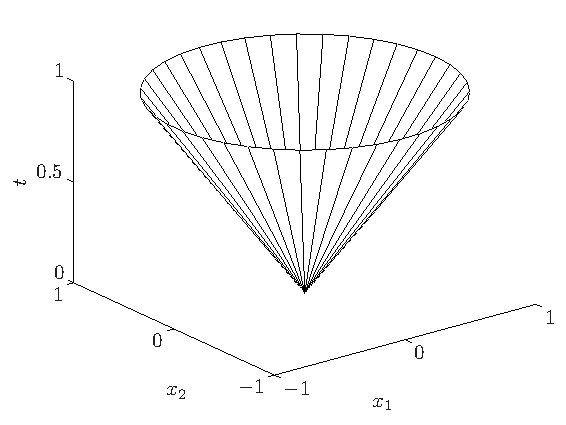
\includegraphics[width=.70\textwidth]{figures/ch02-figure-10.pdf}
\caption*{图2.10\quad $\R^3$ 中二阶锥 $\{(x_1,x_2,t)\mid(x_1^2+x_2^2)^{1/2}\le t\}$ 的边界。}
\end{figure}
顾名思义，范数锥是一个凸锥。

\begin{origexample}{2.3}
\emph{二阶锥}是欧几里得范数对应的范数锥，即
\[
\begin{aligned}
 C&=\{(x,t)\in\R^{n+1}\mid\norm x_2\le t\}\\
 &=\left\{\begin{bmatrix}x\\t\end{bmatrix}\ \middle|\
 \begin{bmatrix}x\\t\end{bmatrix}^{\T}
 \begin{bmatrix}I&0\\0&-1\end{bmatrix}
 \begin{bmatrix}x\\t\end{bmatrix}\le0,\ t\ge0\right\}.
\end{aligned}
\]
二阶锥还有其他几个名称。由于它由二次不等式定义，也称\emph{二次锥}；还称为\emph{Lorentz锥}或\emph{冰淇淋锥}。图2.10给出 $\R^3$ 中的二阶锥。
\end{origexample}

\subsection{多面体}
\emph{多面体}定义为有限个线性等式和线性不等式的解集：
\begin{equation}
 \mathcal P=\{x\mid a_j^{\T}x\le b_j,\ j=1,\ldots,m,
 \ c_j^{\T}x=d_j,\ j=1,\ldots,p\}.\tag{2.5}
\end{equation}
因此，多面体是有限个半空间和超平面的交。仿射集，例如子空间、超平面、直线，以及射线、线段、半空间，都是多面体。容易证明多面体为凸集。有界多面体有时称为多胞体，但有些作者使用相反的约定：将所有（2.5）形式的集合称为多胞体，将其中有界的集合称为多面体。图2.11是五个半空间相交形成的多面体。

% Source PDF page 46 (printed p. 32)
\begin{figure}[htbp]\centering
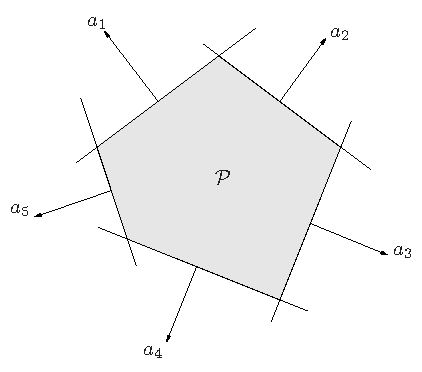
\includegraphics[width=.60\textwidth]{figures/ch02-figure-11.pdf}
\caption*{图2.11\quad 多面体 $\mathcal P$（阴影）是五个半空间的交，外法向量分别为 $a_1,\ldots,a_5$。}
\end{figure}
将（2.5）写成紧凑形式会更方便：
\begin{equation}
 \mathcal P=\{x\mid Ax\preceq b,\ Cx=d\},\tag{2.6}
\end{equation}
其中
\[
 A=\begin{bmatrix}a_1^{\T}\\\vdots\\a_m^{\T}\end{bmatrix},
 \qquad C=\begin{bmatrix}c_1^{\T}\\\vdots\\c_p^{\T}\end{bmatrix}.
\]
符号 $\preceq$ 表示 $\R^m$ 中的向量不等式或逐分量不等式：$u\preceq v$ 的意思是，对 $i=1,\ldots,m$，都有 $u_i\le v_i$。

\begin{origexample}{2.4}
\emph{非负正交锥}是各分量非负的点所成的集合，即
\[
 \R_+^n=\{x\in\R^n\mid x_i\ge0,\ i=1,\ldots,n\}
 =\{x\in\R^n\mid x\succeq0\}.
\]
这里 $\R_+$ 表示非负数集，即 $\R_+=\{x\in\R\mid x\ge0\}$。非负正交锥既是多面体又是锥，因此称为\emph{多面锥}。
\end{origexample}

\subsubsection*{单纯形}
单纯形是另一族重要的多面体。设 $k+1$ 个点 $v_0,\ldots,v_k\in\R^n$ 仿射无关，即 $v_1-v_0,\ldots,v_k-v_0$ 线性无关。由这些点确定的\emph{单纯形}为
\begin{equation}
 C=\conv\{v_0,\ldots,v_k\}
 =\{\theta_0v_0+\cdots+\theta_kv_k\mid\theta\succeq0,\ \one^{\T}\theta=1\}.\tag{2.7}
\end{equation}

% Source PDF page 47 (printed p. 33)
这里 $\one$ 表示各元素均为一的向量。这个单纯形的仿射维数为 $k$，因此有时称为 $\R^n$ 中的 $k$ 维单纯形。

\begin{origexample}{2.5}
\textbf{几个常见的单纯形。}一维单纯形是线段；二维单纯形是三角形及其内部；三维单纯形是四面体。

\emph{单位单纯形}是由零向量与单位向量 $0,e_1,\ldots,e_n\in\R^n$ 确定的 $n$ 维单纯形。它可表示为满足下式的向量集：
\[
 x\succeq0,\qquad\one^{\T}x\le1.
\]
\emph{概率单纯形}是由单位向量 $e_1,\ldots,e_n\in\R^n$ 确定的 $(n-1)$ 维单纯形，即满足
\[
 x\succeq0,\qquad\one^{\T}x=1
\]
的向量集。概率单纯形中的向量对应含 $n$ 个元素的集合上的概率分布，$x_i$ 解释为第 $i$ 个元素的概率。
\end{origexample}

为把单纯形（2.7）描述为多面体，即写成（2.6）的形式，作如下处理。由定义，$x\in C$ 当且仅当存在 $\theta\succeq0$、$\one^{\T}\theta=1$，使 $x=\theta_0v_0+\theta_1v_1+\cdots+\theta_kv_k$。等价地，令 $y=(\theta_1,\ldots,\theta_k)$，且
\[
 B=\begin{bmatrix}v_1-v_0&\cdots&v_k-v_0\end{bmatrix}\in\R^{n\times k},
\]
则 $x\in C$ 当且仅当存在 $y\succeq0$、$\one^{\T}y\le1$，使
\begin{equation}
 x=v_0+By.\tag{2.8}
\end{equation}
点 $v_0,\ldots,v_k$ 仿射无关，意味着 $B$ 的秩为 $k$。因此，存在非奇异矩阵 $A=(A_1,A_2)\in\R^{n\times n}$，使
\[
 AB=\begin{bmatrix}A_1\\A_2\end{bmatrix}B
 =\begin{bmatrix}I\\0\end{bmatrix}.
\]
将（2.8）左乘 $A$，得到
\[
 A_1x=A_1v_0+y,\qquad A_2x=A_2v_0.
\]
因此，$x\in C$ 当且仅当 $A_2x=A_2v_0$，且向量 $y=A_1x-A_1v_0$ 满足 $y\succeq0$、$\one^{\T}y\le1$。换言之，$x\in C$ 当且仅当
\[
 A_2x=A_2v_0,\qquad A_1x\succeq A_1v_0,\qquad
 \one^{\T}A_1x\le1+\one^{\T}A_1v_0.
\]
这些都是关于 $x$ 的线性等式或不等式，因而描述了一个多面体。

% Source PDF page 48 (printed p. 34)
\subsubsection*{多面体的凸包描述}
有限集合 $\{v_1,\ldots,v_k\}$ 的凸包为
\[
 \conv\{v_1,\ldots,v_k\}
 =\{\theta_1v_1+\cdots+\theta_kv_k\mid\theta\succeq0,\ \one^{\T}\theta=1\}.
\]
该集合是有界多面体，但除了单纯形等特殊情况，将它写成（2.5）的形式，也就是用一组线性等式与不等式表示，并不简单。

这种凸包描述的一个推广是
\begin{equation}
 \{\theta_1v_1+\cdots+\theta_kv_k\mid
 \theta_1+\cdots+\theta_m=1,\ \theta_i\ge0,\ i=1,\ldots,k\},\tag{2.9}
\end{equation}
其中 $m\le k$。这里考虑 $v_i$ 的非负线性组合，但只要求前 $m$ 个系数之和为一。也可以把（2.9）解释为点 $v_1,\ldots,v_m$ 的凸包，加上点 $v_{m+1},\ldots,v_k$ 的锥包。集合（2.9）定义一个多面体；反过来，每个多面体都能写成这种形式，尽管这里不作证明。

多面体的表示方式是一个微妙的问题，对实际计算有重要影响。例如，考虑 $\R^n$ 中 $\ell_\infty$ 范数的单位球
\[
 C=\{x\mid\abs{x_i}\le1,\ i=1,\ldots,n\}.
\]
用（2.5）的形式，可以通过 $2n$ 个线性不等式 $\pm e_i^{\T}x\le1$ 描述 $C$，其中 $e_i$ 是第 $i$ 个单位向量。但要用凸包形式（2.9）描述，至少需要 $2^n$ 个点：
\[
 C=\conv\{v_1,\ldots,v_{2^n}\},
\]
其中 $v_1,\ldots,v_{2^n}$ 是所有分量取值为 $1$ 或 $-1$ 的 $2^n$ 个向量。因此，当 $n$ 很大时，这两种描述的规模相差很大。

\subsection{半正定锥}
用 $\mathbf S^n$ 表示对称 $n\times n$ 矩阵集，
\[
 \mathbf S^n=\{X\in\R^{n\times n}\mid X=X^{\T}\},
\]
它是维数为 $n(n+1)/2$ 的向量空间。用 $\mathbf S_+^n$ 表示对称半正定矩阵集，
\[
 \mathbf S_+^n=\{X\in\mathbf S^n\mid X\succeq0\},
\]
用 $\mathbf S_{++}^n$ 表示对称正定矩阵集，
\[
 \mathbf S_{++}^n=\{X\in\mathbf S^n\mid X\succ0\}.
\]
这组记号意在与表示非负实数的 $\R_+$、表示正实数的 $\R_{++}$ 类比。

% Source PDF page 49 (printed p. 35)
\begin{figure}[htbp]\centering
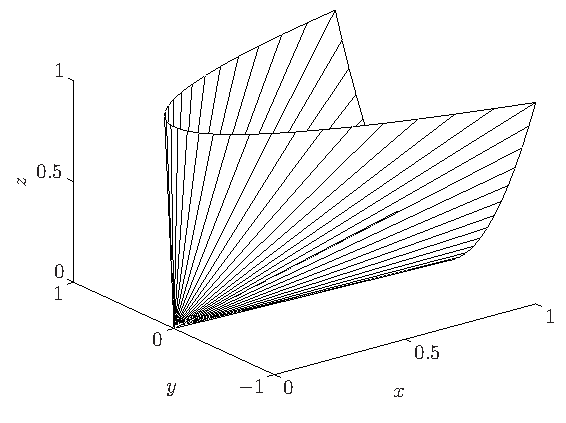
\includegraphics[width=.70\textwidth]{figures/ch02-figure-12.pdf}
\caption*{图2.12\quad $\mathbf S^2$ 中半正定锥的边界。}
\end{figure}
集合 $\mathbf S_+^n$ 是凸锥：如果 $\theta_1,\theta_2\ge0$，且 $A,B\in\mathbf S_+^n$，则 $\theta_1A+\theta_2B\in\mathbf S_+^n$。这可由半正定性的定义直接得到：对任意 $x\in\R^n$，若 $A\succeq0$、$B\succeq0$ 且 $\theta_1,\theta_2\ge0$，则
\[
 x^{\T}(\theta_1A+\theta_2B)x
 =\theta_1x^{\T}Ax+\theta_2x^{\T}Bx\ge0.
\]

\begin{origexample}{2.6}
\textbf{$\mathbf S^2$ 中的半正定锥。}有
\[
 X=\begin{bmatrix}x&y\\y&z\end{bmatrix}\in\mathbf S_+^2
 \quad\Longleftrightarrow\quad x\ge0,\quad z\ge0,\quad xz\ge y^2.
\]
图2.12将 $(x,y,z)$ 画在 $\R^3$ 中，展示了这个锥的边界。
\end{origexample}

\section{保持凸性的运算}
本节介绍一些保持集合凸性的运算，以及由已有凸集构造新凸集的运算。这些运算与第2.2节中的简单例子一起，构成一套凸集运算规则，可用于判断或证明集合的凸性。

% Source PDF page 50 (printed p. 36)
\subsection{交集}
交运算保持凸性：如果 $S_1$ 和 $S_2$ 凸，那么 $S_1\cap S_2$ 凸。该性质可推广到无穷多个集合的交：若对每个 $\alpha\in\mathcal A$，$S_\alpha$ 都凸，则 $\bigcap_{\alpha\in\mathcal A}S_\alpha$ 凸。子空间、仿射集和凸锥也都对任意交运算封闭。一个简单例子是，多面体为半空间和超平面的交，而后者均凸，因此多面体凸。

\begin{origexample}{2.7}
半正定锥 $\mathbf S_+^n$ 可写成
\[
 \bigcap_{z\ne0}\{X\in\mathbf S^n\mid z^{\T}Xz\ge0\}.
\]
对每个 $z\ne0$，$z^{\T}Xz$ 是 $X$ 的一个不恒为零的线性函数，因此集合
\[
 \{X\in\mathbf S^n\mid z^{\T}Xz\ge0\}
\]
实际上是 $\mathbf S^n$ 中的半空间。半正定锥是无穷多个半空间的交，所以凸。
\end{origexample}

\begin{origexample}{2.8}
考虑集合
\begin{equation}
 S=\{x\in\R^m\mid\abs{p(t)}\le1,\ \abs t\le\pi/3\},\tag{2.10}
\end{equation}
其中 $p(t)=\sum_{k=1}^m x_k\cos kt$。集合 $S$ 可以表示为无穷多个带状区域的交 $S=\bigcap_{\abs t\le\pi/3}S_t$，其中
\[
 S_t=\{x\mid-1\le(\cos t,\ldots,\cos mt)^{\T}x\le1\},
\]
所以凸。图2.13和图2.14展示了 $m=2$ 时的定义及相应集合。
\end{origexample}

上面的例子将集合表示为可能无穷多个半空间的交，从而证明其凸性。第2.5.1节将看到，反过来也成立：每个闭凸集 $S$ 都是若干半空间的交，通常需要无穷多个。事实上，闭凸集 $S$ 等于所有包含它的半空间的交：
\[
 S=\bigcap\{H\mid H\text{ 为半空间},\ S\subseteq H\}.
\]

\subsection{仿射函数}
回顾，函数 $f:\R^n\to\R^m$ 若是线性函数与常数的和，就称为仿射函数，也就是具有形式 $f(x)=Ax+b$，其中 $A\in\R^{m\times n}$、$b\in\R^m$。若 $S\subseteq\R^n$ 凸，$f:\R^n\to\R^m$ 仿射，则 $S$ 在 $f$ 下的像
\[
 f(S)=\{f(x)\mid x\in S\}
\]
为凸集。

% Source PDF page 51 (printed p. 37)
\begin{figure}[htbp]\centering
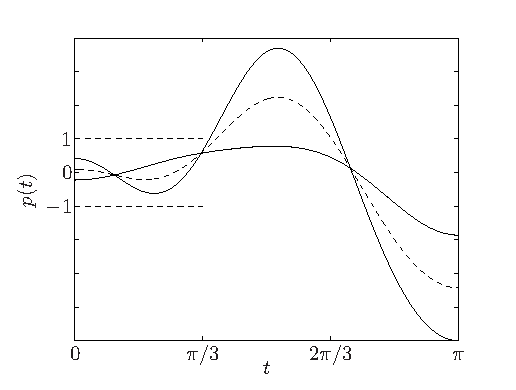
\includegraphics[width=.72\textwidth]{figures/ch02-figure-13.pdf}
\caption*{图2.13\quad （2.10）中 $m=2$ 时，与集合 $S$ 中三个点相应的三角多项式。虚线表示的三角多项式是另外两个的平均。}
\end{figure}
\begin{figure}[htbp]\centering
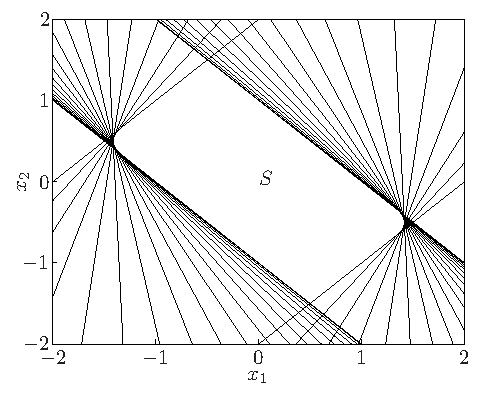
\includegraphics[width=.63\textwidth]{figures/ch02-figure-14.pdf}
\caption*{图2.14\quad （2.10）中 $m=2$ 时的集合 $S$，为图中央的白色区域。它是无穷多个带状区域的交，图中画出了其中20个，因此为凸集。}
\end{figure}

% Source PDF page 52 (printed p. 38)
类似地，若 $f:\R^k\to\R^n$ 仿射，则 $S$ 在 $f$ 下的逆像
\[
 f^{-1}(S)=\{x\mid f(x)\in S\}
\]
也凸。

两个简单例子是缩放和平移。若 $S\subseteq\R^n$ 凸，$\alpha\in\R$、$a\in\R^n$，则 $\alpha S$ 和 $S+a$ 都凸，其中
\[
 \alpha S=\{\alpha x\mid x\in S\},\qquad S+a=\{x+a\mid x\in S\}.
\]
凸集投影到部分坐标所得的集合也凸：若 $S\subseteq\R^m\times\R^n$ 凸，则
\[
 T=\{x_1\in\R^m\mid\text{存在 }x_2\in\R^n,\ (x_1,x_2)\in S\}
\]
凸。

两个集合的\emph{和}定义为
\[
 S_1+S_2=\{x+y\mid x\in S_1,\ y\in S_2\}.
\]
若 $S_1$ 和 $S_2$ 凸，则 $S_1+S_2$ 凸。因为当 $S_1$ 和 $S_2$ 凸时，它们的直积或笛卡尔积
\[
 S_1\times S_2=\{(x_1,x_2)\mid x_1\in S_1,\ x_2\in S_2\}
\]
也凸，而该集合在线性函数 $f(x_1,x_2)=x_1+x_2$ 下的像，正是 $S_1+S_2$。

还可以考虑 $S_1,S_2\in\R^n\times\R^m$ 的\emph{部分和}，定义为
\[
 S=\{(x,y_1+y_2)\mid(x,y_1)\in S_1,\ (x,y_2)\in S_2\},
\]
其中 $x\in\R^n$、$y_i\in\R^m$。$m=0$ 时，部分和给出 $S_1$ 和 $S_2$ 的交；$n=0$ 时，它就是集合加法。凸集的部分和仍凸，见习题2.16。

\begin{origexample}{2.9}
\textbf{多面体。}多面体 $\{x\mid Ax\preceq b,\ Cx=d\}$ 可写成非负正交锥与原点的笛卡尔积在仿射函数 $f(x)=(b-Ax,d-Cx)$ 下的逆像：
\[
 \{x\mid Ax\preceq b,\ Cx=d\}
 =\{x\mid f(x)\in\R_+^m\times\{0\}\}.
\]
\end{origexample}

\begin{origexample}{2.10}
\textbf{线性矩阵不等式的解集。}条件
\begin{equation}
 A(x)=x_1A_1+\cdots+x_nA_n\preceq B,\tag{2.11}
\end{equation}
其中 $B,A_i\in\mathbf S^m$，称为关于 $x$ 的\emph{线性矩阵不等式}（LMI）。注意，它与普通线性不等式
\[
 a^{\T}x=x_1a_1+\cdots+x_na_n\le b
\]
类似，后者的 $b,a_i\in\R$。

线性矩阵不等式的解集 $\{x\mid A(x)\preceq B\}$ 是凸集。事实上，它是半正定锥在仿射函数 $f:\R^n\to\mathbf S^m$，$f(x)=B-A(x)$ 下的逆像。
\end{origexample}

% Source PDF page 53 (printed p. 39)
\begin{origexample}{2.11}
\textbf{双曲锥。}集合
\[
 \{x\mid x^{\T}Px\le(c^{\T}x)^2,\ c^{\T}x\ge0\},
\]
其中 $P\in\mathbf S_+^n$、$c\in\R^n$，为凸集，因为它是二阶锥
\[
 \{(z,t)\mid z^{\T}z\le t^2,\ t\ge0\}
\]
在仿射函数 $f(x)=(P^{1/2}x,c^{\T}x)$ 下的逆像。
\end{origexample}

\begin{origexample}{2.12}
\textbf{椭球。}椭球
\[
 \mathcal E=\{x\mid(x-x_c)^{\T}P^{-1}(x-x_c)\le1\},
\]
其中 $P\in\mathbf S_{++}^n$，是单位欧几里得球 $\{u\mid\norm u_2\le1\}$ 在仿射映射 $f(u)=P^{1/2}u+x_c$ 下的像。它也是单位球在仿射映射 $g(x)=P^{-1/2}(x-x_c)$ 下的逆像。
\end{origexample}

\subsection{线性分式函数与透视函数}
本节研究一类比仿射函数更一般、但仍保持凸性的函数，称为\emph{线性分式函数}。

\subsubsection*{透视函数}
定义\emph{透视函数} $P:\R^{n+1}\to\R^n$，其定义域为 $\dom P=\R^n\times\R_{++}$，函数值为 $P(z,t)=z/t$。这里 $\R_{++}=\{x\in\R\mid x>0\}$ 为正数集。透视函数缩放或归一化向量，使最后一个分量等于一，再去掉最后一个分量。

\begin{quote}\textbf{说明2.1}\quad
可以把透视函数理解为针孔相机的作用。$\R^3$ 中的针孔相机由不透光水平面 $x_3=0$ 构成，原点处有一个允许光线通过的针孔，水平像平面为 $x_3=-1$。相机上方，即 $x_3>0$ 处，位于 $x$ 的物体，在像平面上的点 $-(x_1/x_3,x_2/x_3,1)$ 处成像。去掉恒为 $-1$ 的最后一个分量，物体 $x$ 的像在像平面上的位置就是 $y=-(x_1/x_3,x_2/x_3)=-P(x)$，见图2.15。
\end{quote}
若 $C\subseteq\dom P$ 凸，则其像
\[
 P(C)=\{P(x)\mid x\in C\}
\]
也凸。这个结果符合直觉：通过针孔相机观察凸物体，会得到凸的像。为证明这一点，我们说明透视函数将线段映射为线段。这也符合直觉：通过针孔相机观察线段，得到的像仍是线段。

% Source PDF page 54 (printed p. 40)
\begin{figure}[htbp]\centering
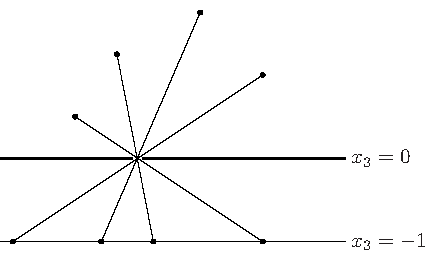
\includegraphics[width=.65\textwidth]{figures/ch02-figure-15.pdf}
\caption*{图2.15\quad 透视函数的针孔相机解释。深色水平线表示 $\R^3$ 中不透光的平面 $x_3=0$，只在原点有针孔。平面上方的物体或光源在较浅水平线表示的像平面 $x_3=-1$ 上成像。光源位置到像位置的映射与透视函数有关。}
\end{figure}
设 $x=(\widetilde x,x_{n+1})$、$y=(\widetilde y,y_{n+1})\in\R^{n+1}$，且 $x_{n+1}>0$、$y_{n+1}>0$。对 $0\le\theta\le1$，有
\[
 P(\theta x+(1-\theta)y)
 =\frac{\theta\widetilde x+(1-\theta)\widetilde y}
 {\theta x_{n+1}+(1-\theta)y_{n+1}}
 =\mu P(x)+(1-\mu)P(y),
\]
其中
\[
 \mu=\frac{\theta x_{n+1}}
 {\theta x_{n+1}+(1-\theta)y_{n+1}}\in[0,1].
\]
$\theta$ 与 $\mu$ 的对应关系是单调的：当 $\theta$ 在0与1之间变化，遍历线段 $[x,y]$ 时，$\mu$ 也在0与1之间变化，遍历线段 $[P(x),P(y)]$。因此，$P([x,y])=[P(x),P(y)]$。

现在，设 $C$ 凸且 $C\subseteq\dom P$，即对每个 $x\in C$ 都有 $x_{n+1}>0$，并取 $x,y\in C$。为证明 $P(C)$ 凸，只需说明线段 $[P(x),P(y)]$ 在 $P(C)$ 中。该线段是 $[x,y]$ 在 $P$ 下的像，因而确实包含在 $P(C)$ 中。

凸集在透视函数下的逆像也凸：若 $C\subseteq\R^n$ 凸，则
\[
 P^{-1}(C)=\{(x,t)\in\R^{n+1}\mid x/t\in C,\ t>0\}
\]
凸。为证明这一点，设 $(x,t)\in P^{-1}(C)$、$(y,s)\in P^{-1}(C)$，且 $0\le\theta\le1$。需要说明
\[
 \theta(x,t)+(1-\theta)(y,s)\in P^{-1}(C),
\]
即
\[
 \frac{\theta x+(1-\theta)y}{\theta t+(1-\theta)s}\in C.
\]
